% Story mode, proposed: eight chapters along the road, each a short run of
% scenes, after Super Smash Bros. Melee's Adventure Mode (twelve stages that
% mix a stage to cross with matches of several kinds).
% Chapter names are road.region.* in data/copy.en.json; scene kinds are the
% proposal's (analysis/story/PROPOSAL.md). Standalone: compiles with pdflatex.
\documentclass[tikz,border=4pt]{standalone}
\usetikzlibrary{arrows.meta,positioning,calc}

% --- Colors: the game's palette (data/palette.json) --------------------------
\definecolor{paper}{HTML}{EFE8D8}   % background
\definecolor{ink}{HTML}{2B2A28}     % text and lines
\definecolor{muted}{HTML}{6B6457}   % secondary text
\definecolor{indigo}{HTML}{3E4A89}  % the player's color
\definecolor{ochre}{HTML}{B8862B}   % the opponents' color
\definecolor{ground}{HTML}{D9CDB2}  % chapter cards
% One color per scene kind (the legend at the bottom names them)
\definecolor{kduel}{HTML}{2B2A28}
\definecolor{kcross}{HTML}{3E4A89}
\definecolor{khorde}{HTML}{B8862B}
\definecolor{kteam}{HTML}{2A6B4A}
\definecolor{ksurvive}{HTML}{6B6457}
\definecolor{kgiant}{HTML}{7A5618}

% --- Layout, in centimetres --------------------------------------------------
\newcommand{\CardW}{6.2}   % chapter card width
\newcommand{\CardH}{4.6}   % chapter card height
\newcommand{\Gap}{1.3}     % space between cards
\newcommand{\RowGap}{2.2}  % space between the two rows

\begin{document}
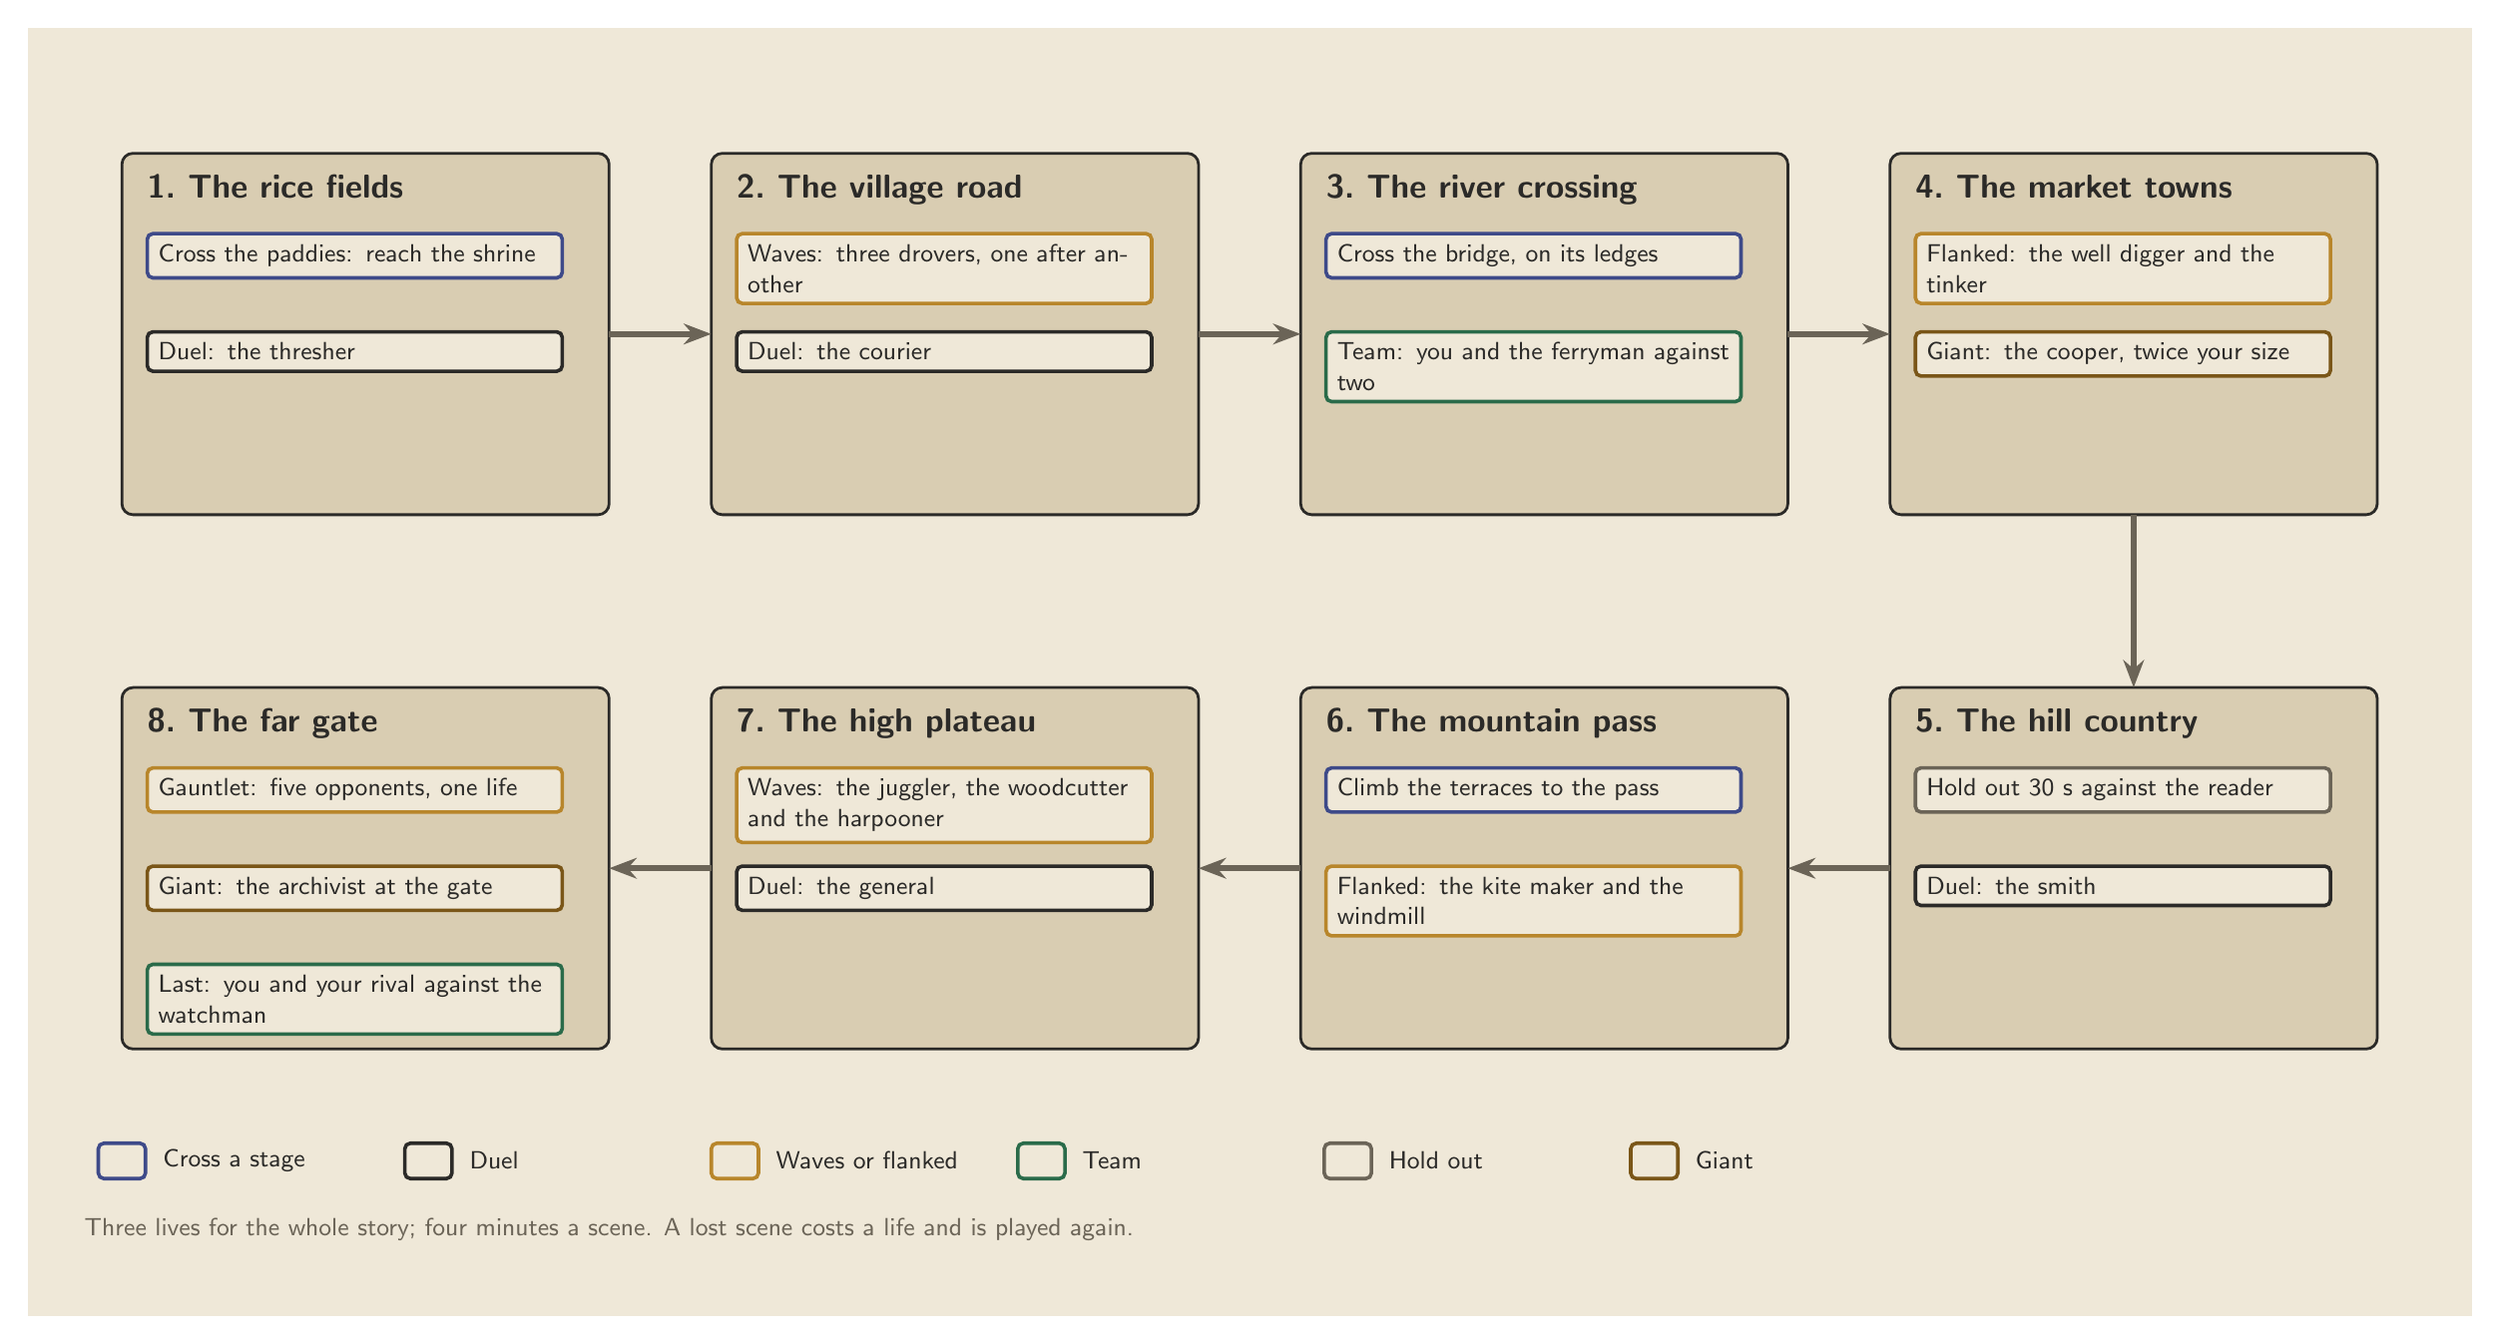
\begin{tikzpicture}[font=\sffamily, ink,
    card/.style={draw=ink, line width=1pt, fill=ground, rounded corners=4pt},
    scene/.style={draw=#1, line width=1.3pt, fill=paper, rounded corners=2pt, text width=5.0cm, align=left, inner sep=4pt, font=\sffamily\small},
    road/.style={-{Stealth[length=3.5mm]}, line width=2pt, draw=muted},
  ]
% --- Background ---------------------------------------------------------------
\fill[paper] (-1.2,1.6) rectangle (4*\CardW+3*\Gap+1.2, -2*\CardH-\RowGap-3.4);

% --- Chapters: a name, then its scenes as {kind color}/{text} -------------------
% Row 1 runs left to right, row 2 right to left, so the road snakes.
\foreach \n/\cname/\scenes in {
  1/{The rice fields}/{kcross/{Cross the paddies: reach the shrine}, kduel/{Duel: the thresher}},
  2/{The village road}/{khorde/{Waves: three drovers, one after another}, kduel/{Duel: the courier}},
  3/{The river crossing}/{kcross/{Cross the bridge, on its ledges}, kteam/{Team: you and the ferryman against two}},
  4/{The market towns}/{khorde/{Flanked: the well digger and the tinker}, kgiant/{Giant: the cooper, twice your size}},
  5/{The hill country}/{ksurvive/{Hold out 30 s against the reader}, kduel/{Duel: the smith}},
  6/{The mountain pass}/{kcross/{Climb the terraces to the pass}, khorde/{Flanked: the kite maker and the windmill}},
  7/{The high plateau}/{khorde/{Waves: the juggler, the woodcutter and the harpooner}, kduel/{Duel: the general}},
  8/{The far gate}/{khorde/{Gauntlet: five opponents, one life}, kgiant/{Giant: the archivist at the gate}, kteam/{Last: you and your rival against the watchman}}}
{
  \pgfmathtruncatemacro{\row}{(\n-1)/4}
  \pgfmathtruncatemacro{\col}{mod(\n-1,4)}
  \pgfmathsetmacro{\x}{ifthenelse(\row==0, \col, 3-\col)*(\CardW+\Gap)}
  \pgfmathsetmacro{\y}{-\row*(\CardH+\RowGap)}
  \draw[card] (\x,\y) rectangle ++(\CardW,-\CardH);
  \node[anchor=north west, font=\sffamily\bfseries\large, text width=5.8cm] at (\x+0.2,\y-0.15) {\n.\ \cname};
  \foreach \k/\t [count=\j] in \scenes {
    \node[scene=\k, anchor=north west] at (\x+0.3,\y-1.0-1.25*\j+1.25) {\t};
  }
}

% --- The road between chapters ------------------------------------------------
\foreach \i in {0,1,2} {
  \draw[road] (\i*\CardW+\i*\Gap+\CardW,-\CardH/2) -- ++(\Gap,0);
  \draw[road] (3*\CardW+3*\Gap-\i*\CardW-\i*\Gap,-\CardH-\RowGap-\CardH/2) -- ++(-\Gap,0);
}
\draw[road] (3*\CardW+3*\Gap+\CardW/2,-\CardH) -- ++(0,-\RowGap);

% --- Legend (drawn last) ------------------------------------------------------
\foreach \k/\lbl [count=\m] in {kcross/Cross a stage,kduel/Duel,khorde/Waves or flanked,kteam/Team,ksurvive/Hold out,kgiant/Giant} {
  \draw[line width=1.3pt, draw=\k, fill=paper, rounded corners=2pt] (-0.6+\m*3.9-3.6,-2*\CardH-\RowGap-1.2) rectangle ++(0.6,-0.45);
  \node[anchor=west, font=\sffamily\small] at (-0.6+\m*3.9-2.9,-2*\CardH-\RowGap-1.42) {\lbl};
}
\node[anchor=west, font=\sffamily\small, text=muted] at (-0.6,-2*\CardH-\RowGap-2.3)
  {Three lives for the whole story; four minutes a scene. A lost scene costs a life and is played again.};
\end{tikzpicture}
\end{document}
